\clearpage
\section{Voltage determination}\label{sec:vol}
As first thing, we check the gas system. There are bubbles coming out every few seconds at window on a test tube, it is clear that the gas system was working. Then we need to determine voltages of PMTs and discriminator. 

\subsection{PMT operation voltage determination}
As mentioned in section~\ref{sec:drift}, behaviour of drift chamber strongly depends on voltage applied between anode and cathode. Thus to make sure PMTs are working properly, voltages need to be set accordingly. To determine the PMT operation voltages we have three counters. They show the number of events in \SI{10}{\s} interval of top PMT, bottom PMT, and coincidence of these two.

We start by varying the voltage for bottom panel from \SI{1700}{\volt} to \SI{2300}{\volt} in steps of \SI{50}{\volt}. Four measurements at every \num{10} second with every step of \SI{50}{\volt} and calculate their averages to reduce the statistical errors. After measuring rate, we plot a graph between average rate against number of counts. Errors of "count rates" are estimated using Poisson distribution. In figure \ref{fig:PMTvoltageBot} we can see that initially the count rate increases quite steeply with the voltage. Then it start to get saturated from \SI{2000}{\volt} and flattens out from \SI{2100}{V}. In the this region, a linear fit is done. We see that data points with voltages less or equal to \SI{2050}{\volt} don't follow this linear fit anymore. Therefore. According to~\cite{manual}, we took a working point at starting point of the plateau, thus \SI{2100}{\volt}.

\begin{figure}[H]
\begin{center}
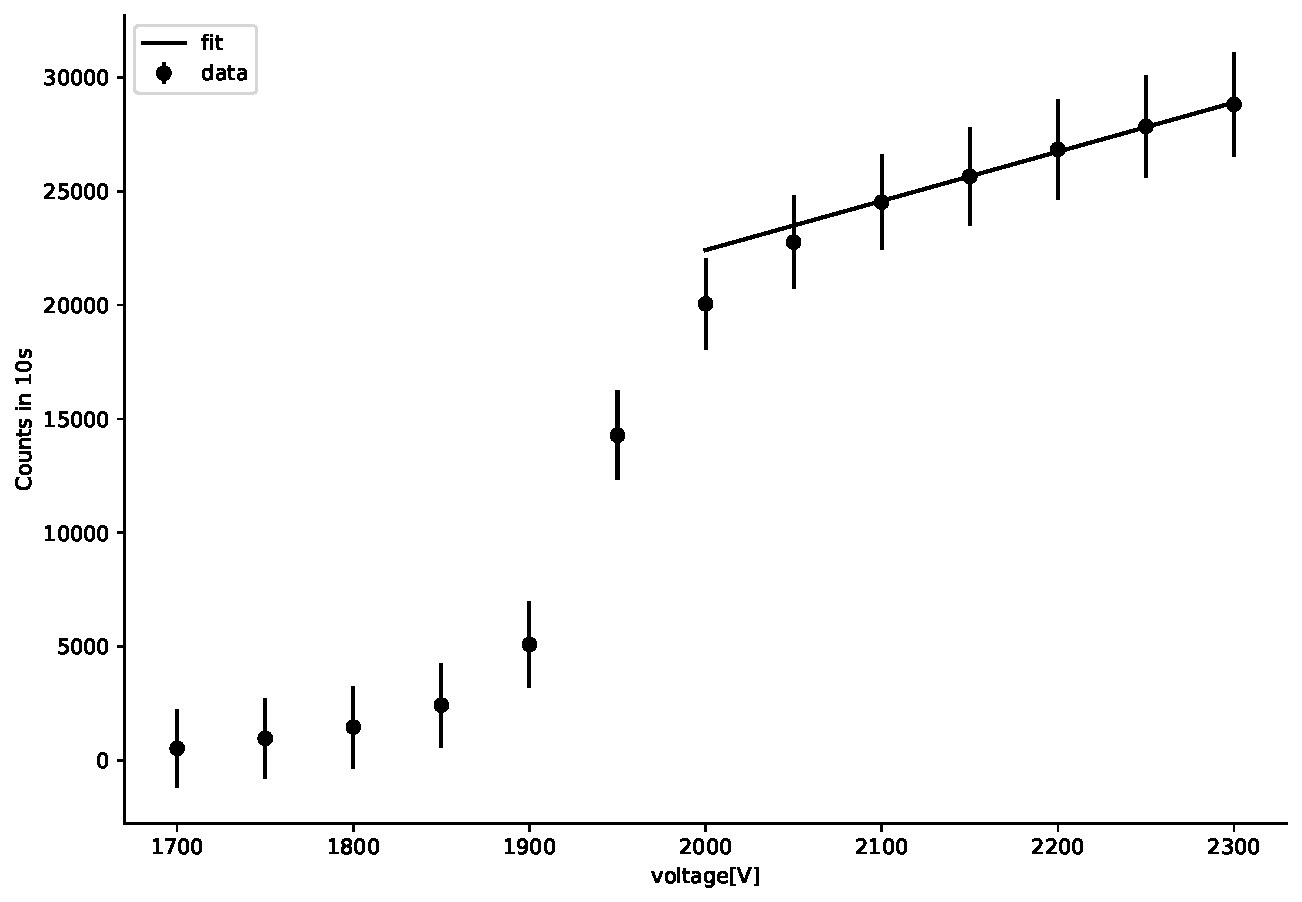
\includegraphics[width=0.6\linewidth]{bot.pdf}
	\end{center}
\caption{The number of counts for bottom panel with varying voltage. Vertical axis is in log scale. Raw data are in appendix.}
\label{fig:PMTvoltageBot}
\end{figure}

With bottom PMT voltage at \SI{2100}{\volt}, we vary the voltage for top panel as in before step in the same range. We measure the coincidence rate via its counter. Unfortunately, the rightmost counter is slightly broken, the last digit of count number is not clearly readable. It could lead some statistical error, but in the end it is not very significant. By plotting a graph of coincidence rate over, we have again a plateau curve \ref{fig:PMTvoltageTop}. From figure \ref{fig:PMTvoltageTop} we see that initially coincidence rate increases with voltage then it has a clear plateau. \SI{2150}{\volt} is the point the curve starts to be flat and it is a good working point for the PMT.
	
\begin{figure}[H]
		\begin{center}
			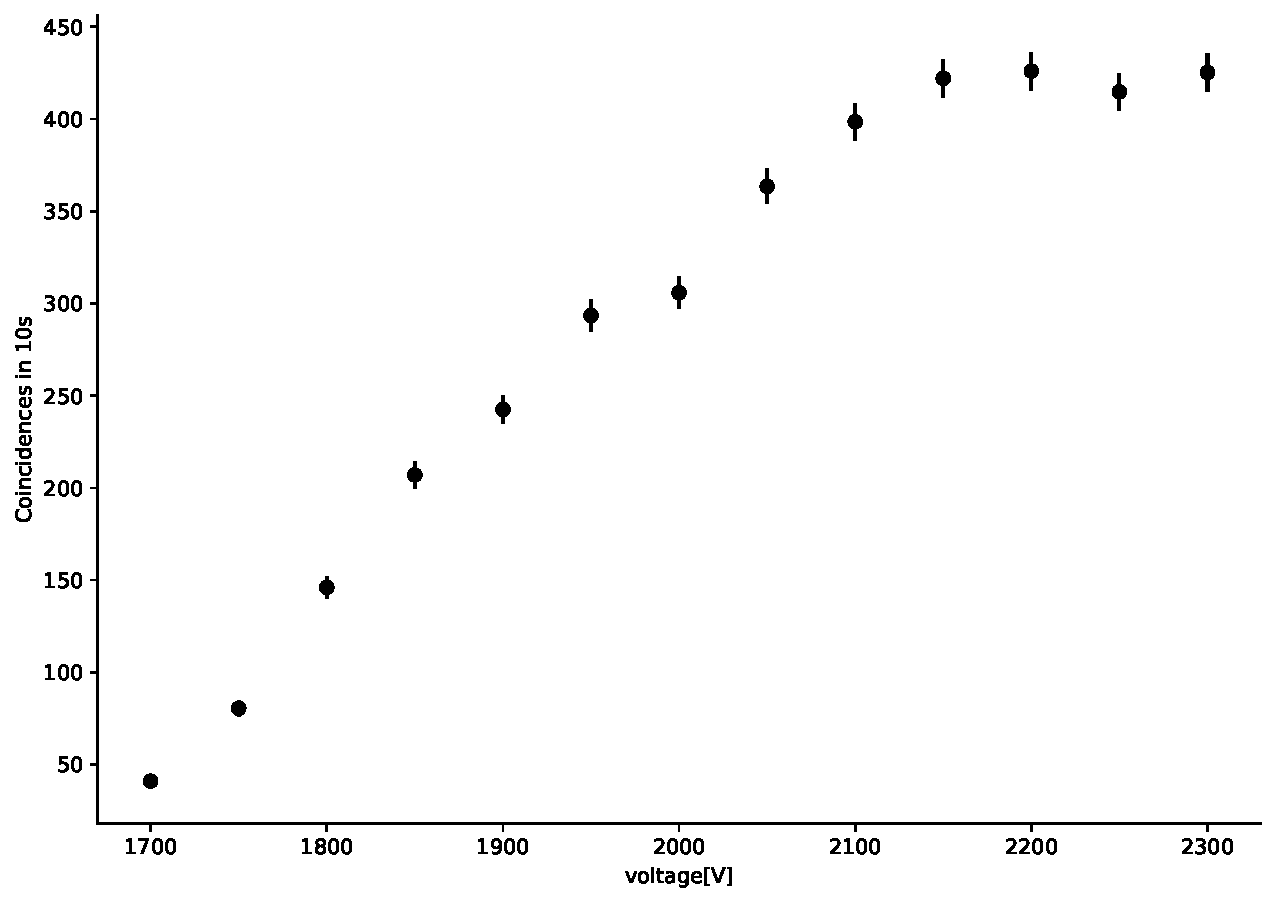
\includegraphics[width=0.6\linewidth]{top.pdf}
		\end{center}
	\caption{The number of counts for top panel with varying voltage. Raw data are in appendix.}%
	\label{fig:PMTvoltageTop}
\end{figure}	
	
\subsection{Determination of the front-end threshold voltage}	
We have to determine the optimal voltage for the discriminator. The voltage is adjusted using power supply \cite{manual}. To determine its appropriate value, we processed with \verb|StyxM2C2| along with the raw data. Here, we have taken \num{25000} events in every step of \SI{0.3}{\volt} from \SI{1.4}{\volt} to \SI{2.6}{\volt}. Then to do find good channels a closer look into the \verb|root| files is necessary.  Finally, we compared the different voltage settings using \verb|StyxThresholdScane|.

To choose threshold voltage, first of all, we look at the rates files two of them are in fig \ref{fig:rate}. The hits in channel decreases with increasing voltage. At low voltages (low threshold) there are plenty of noises and at high voltage some of the signals are cut. So we indeed expect decreasing curves in rate files. Thus we say that roughly the optimal voltage should be in the middle. Its exact value needs still to be determined later.
\begin{figure}[H]
	\centering
	\begin{subfigure}[t]{0.8\textwidth}
		\begin{center}
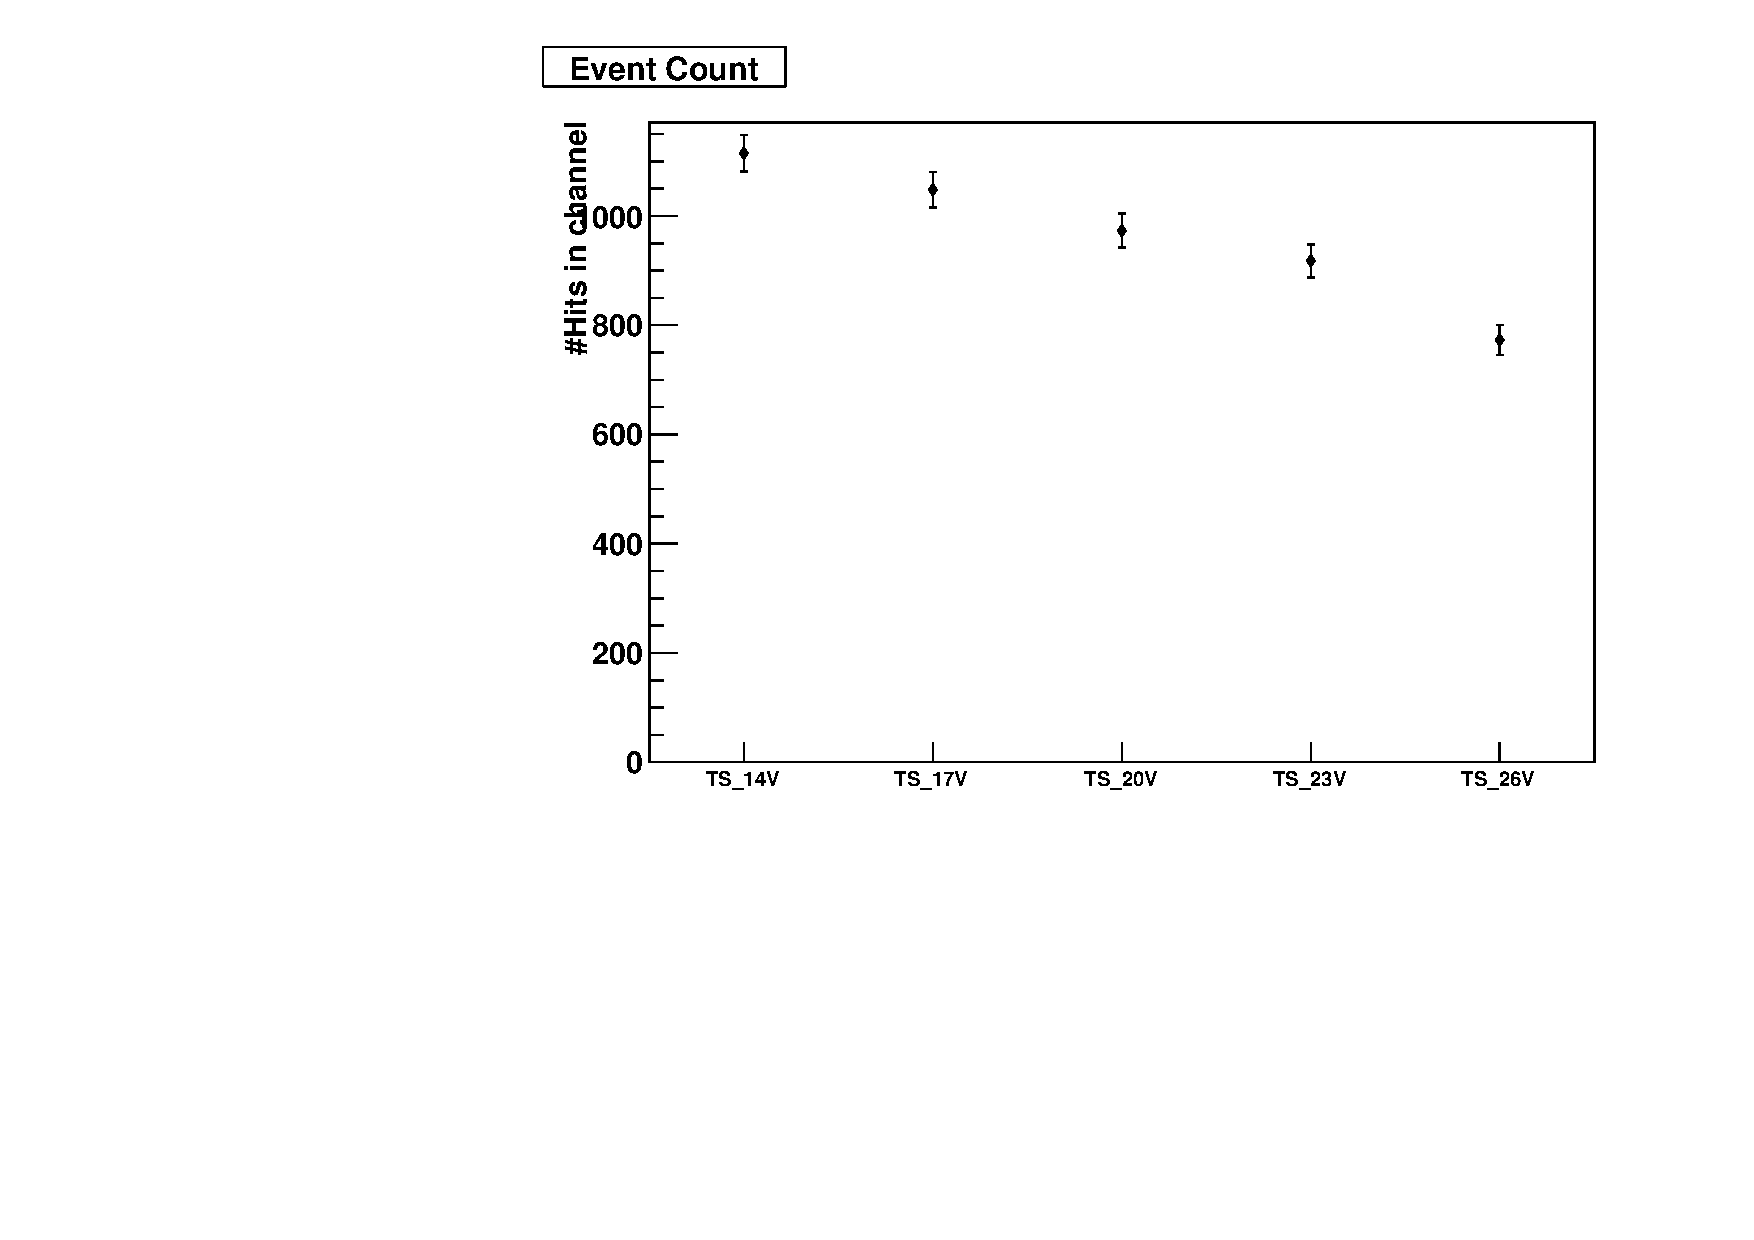
\includegraphics[width=0.8\linewidth]{StyxThresholdScan_1_2_Rate.pdf}
		\end{center}
		\caption{At TDC 1 channel 2.}
	\end{subfigure}
	
	\begin{subfigure}[t]{0.8\textwidth}
		\begin{center}
	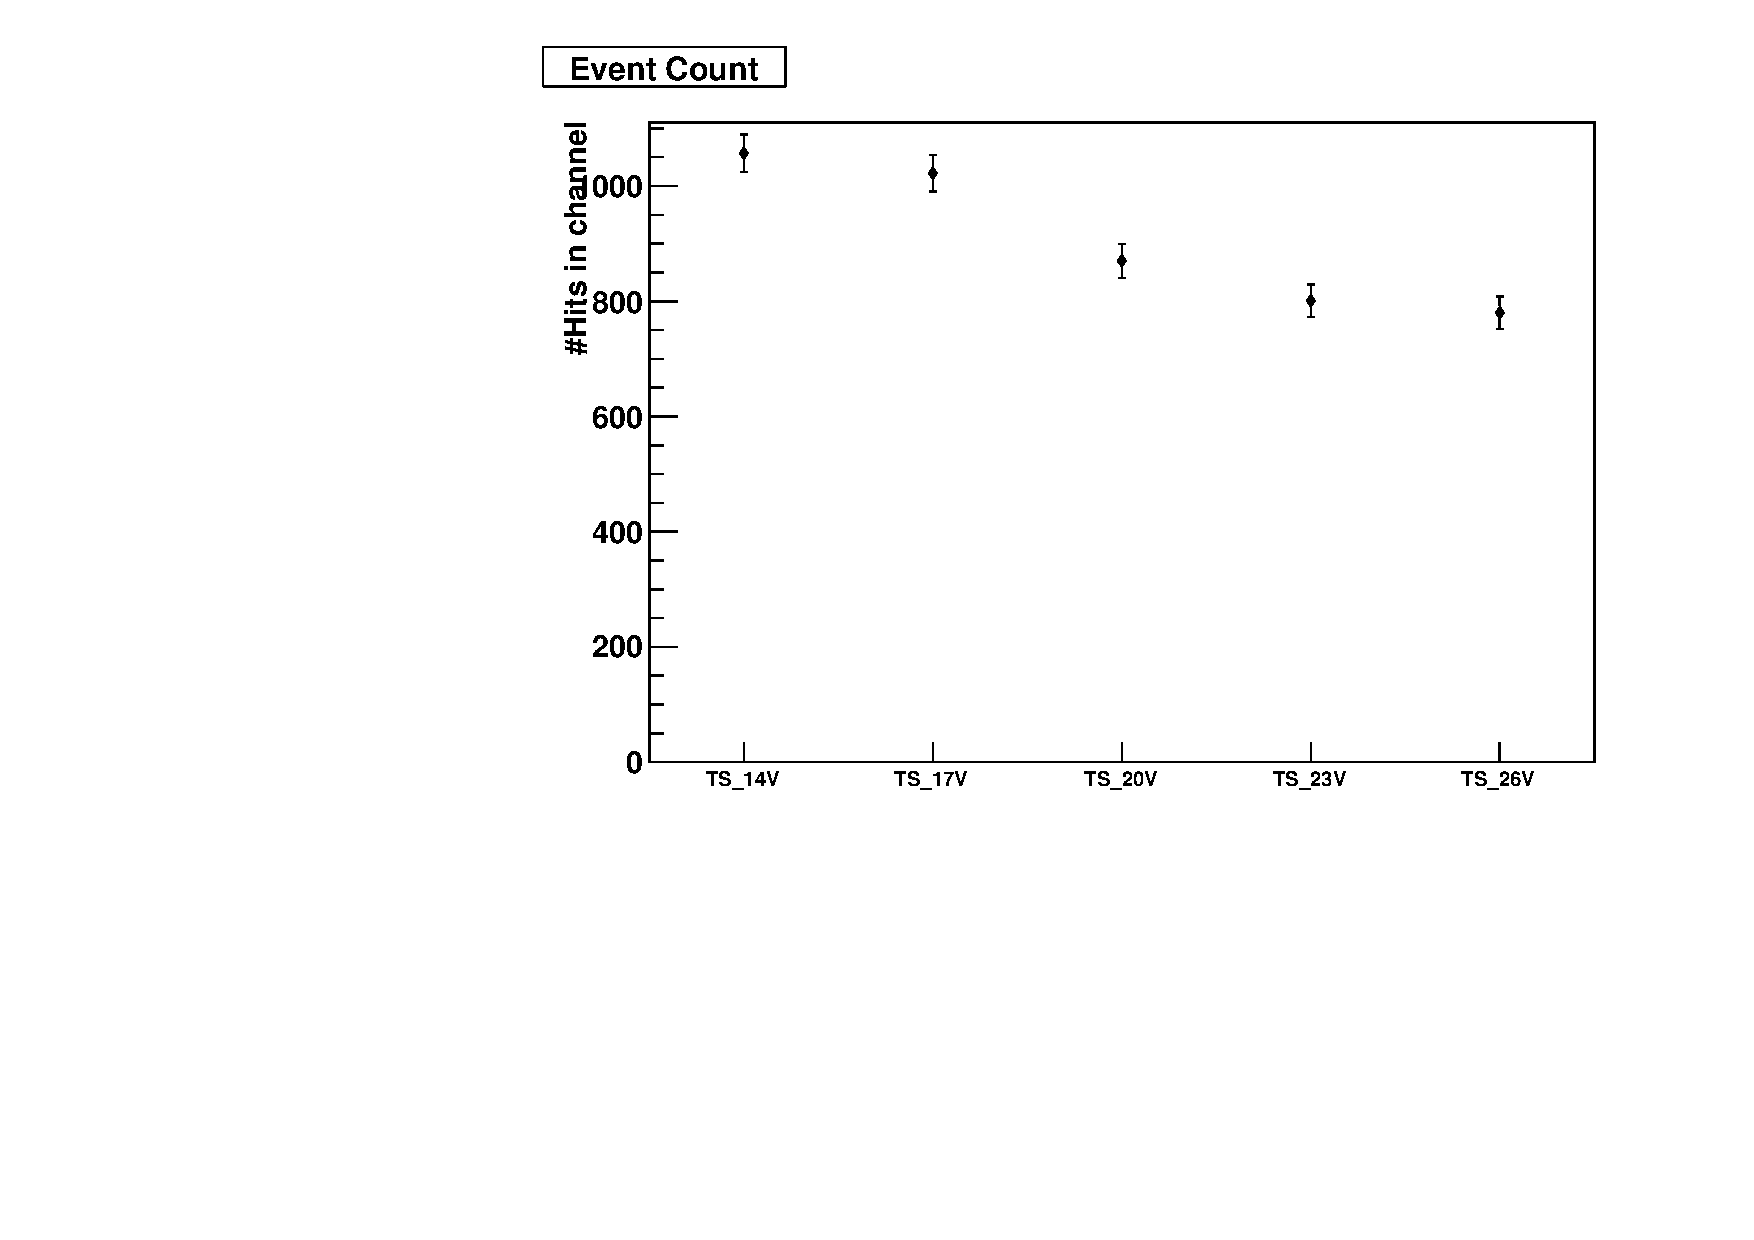
\includegraphics[width=0.8\linewidth]{StyxThresholdScan_1_5_Rate.pdf}
		\end{center}
		\caption{At TDC 1 channel 5.}
	\end{subfigure}
	\caption{The rate plots in TDC 1 channel 2 and TDC 1 channel 5 at different voltages.}%
	\label{fig:rate}
\end{figure}

Now we compare the overlay plots of different channels and TDCs. Two examples are in fig \ref{fig:Overlay}. It shows number of hits in six straws at different voltages. In figure \ref{fig:Overlay}, the peaks are for different straws and horizontal axis is in time which has something to do with electronics of the setup~\cite{manual}. We see that the noise level is too high at low voltages and thus heights of these peaks are quite different. Peaks at \SI{2.0}{\volt} seems quite uniform for all straws, but not for other voltages. We want to find the lowest voltage so that the peaks seem to be of the same heights. Therefore we choose the threshold voltage is \SI{2.0}{\volt}.

\begin{figure}[H]
	\centering
\begin{subfigure}{0.8\textwidth}
 \begin{center}
 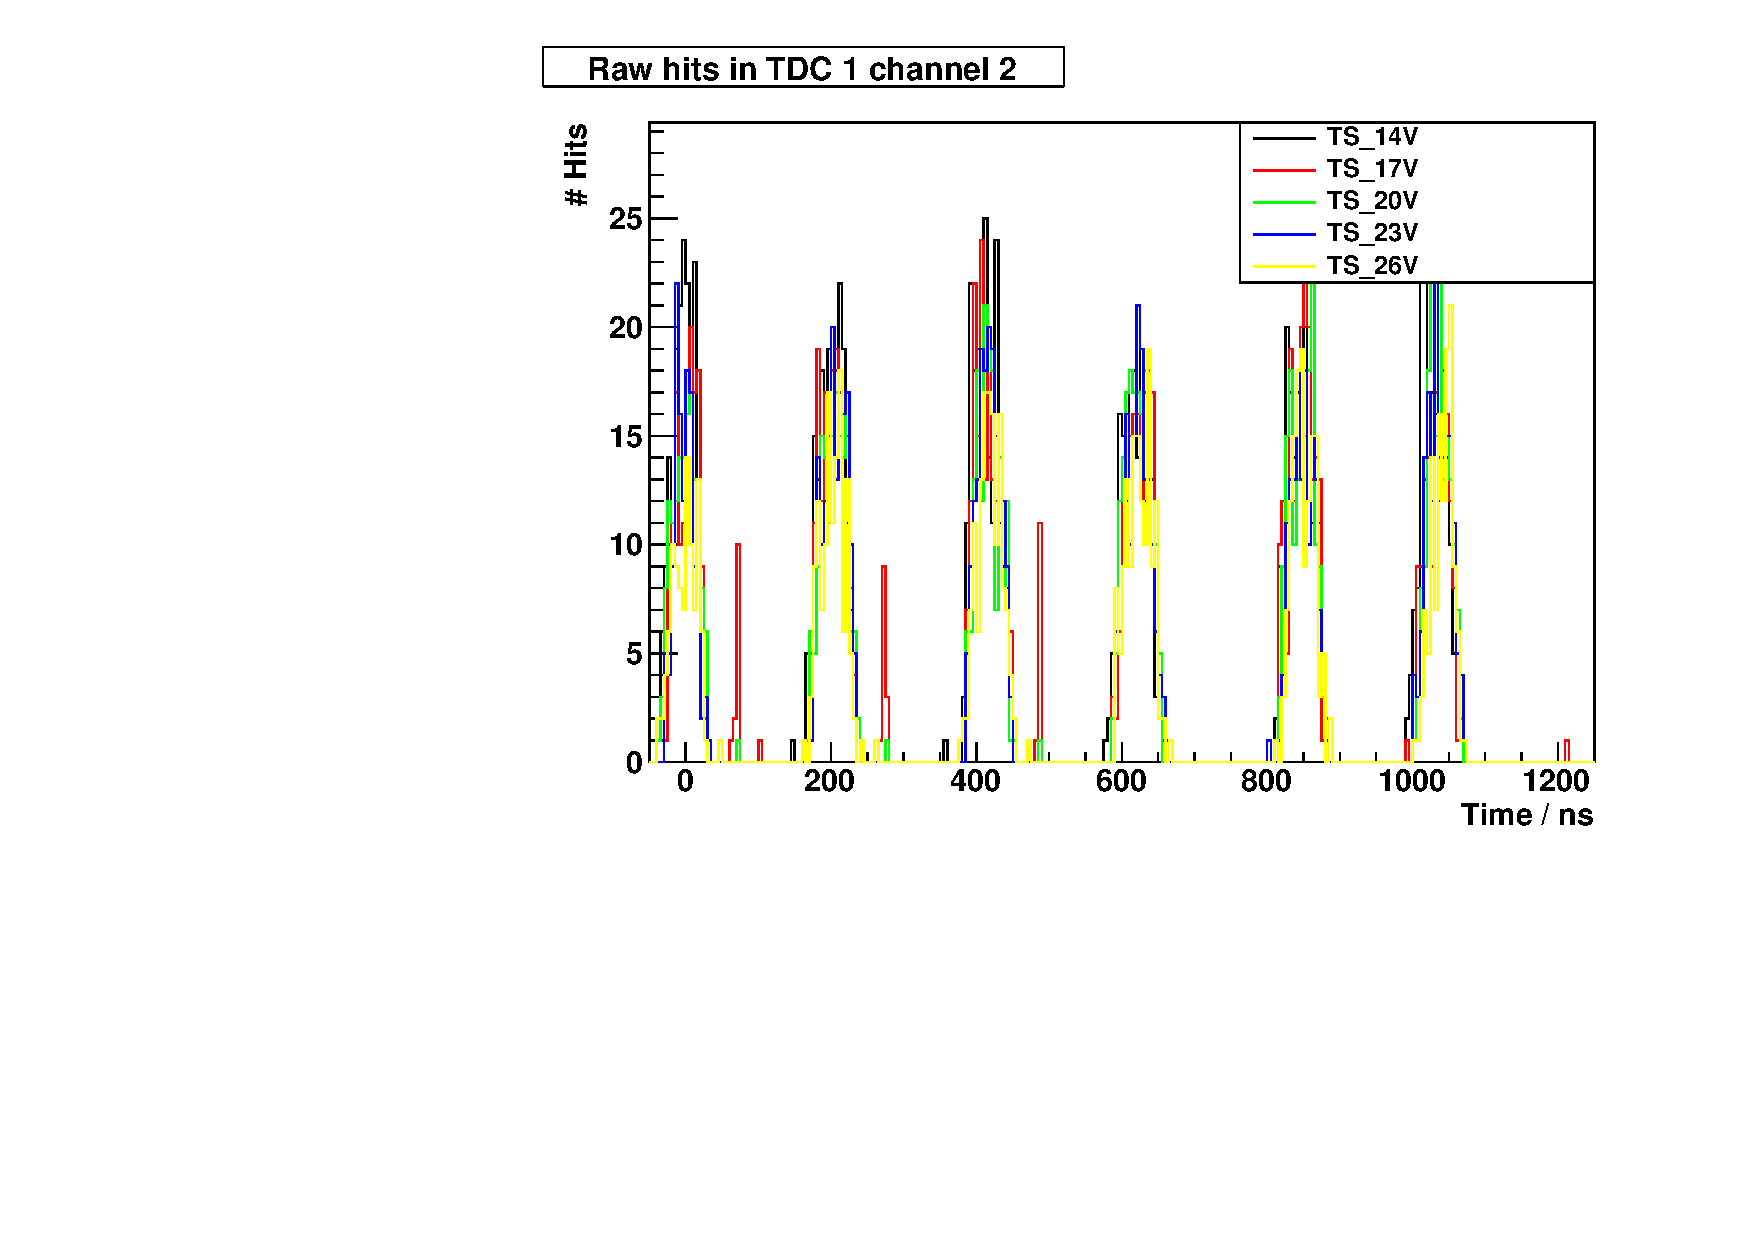
\includegraphics[width=0.8\linewidth]{StyxThresholdScan_1_2_Overlay.pdf}
 \end{center}
 	\caption{In TDC 1 channel 2 at different voltages.}
 \end{subfigure}
 
 \begin{subfigure}{0.8\textwidth}
 	\begin{center}
 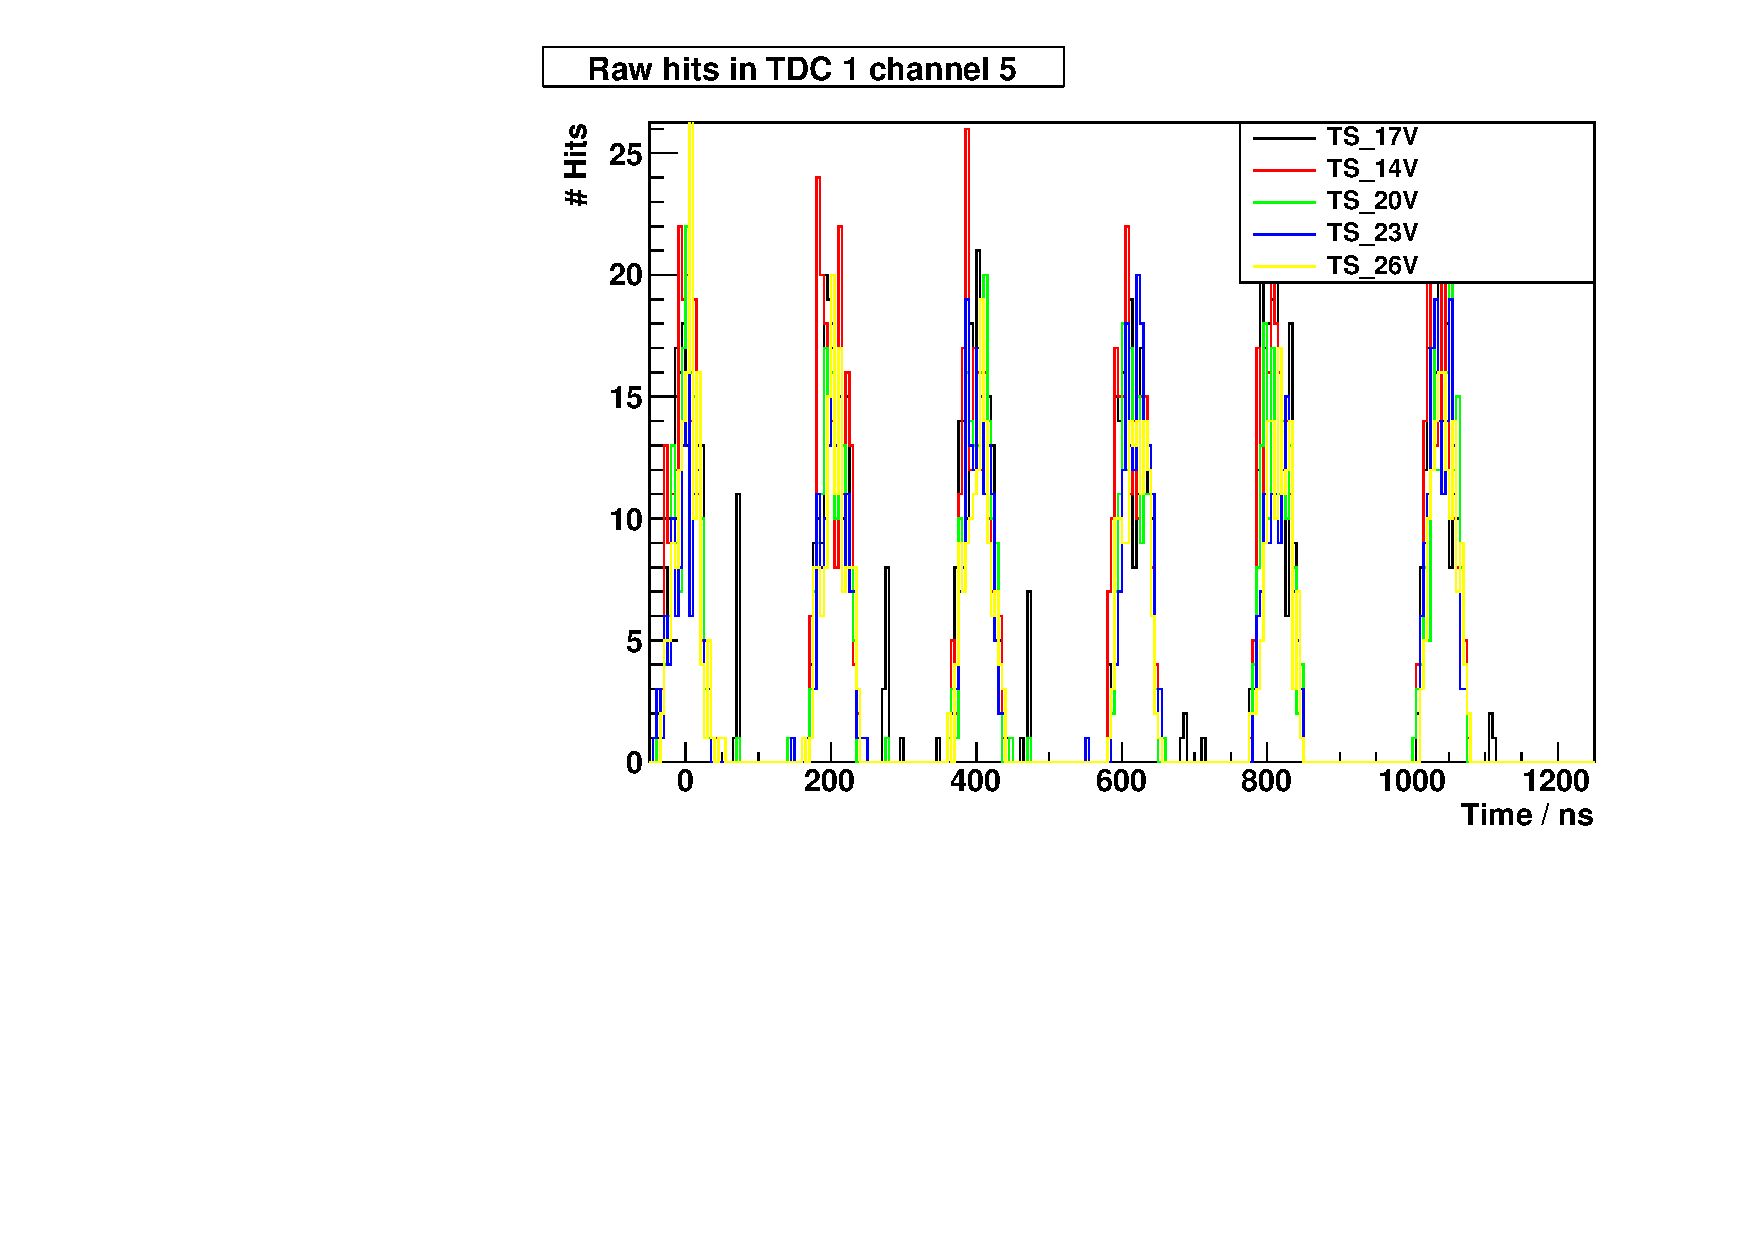
\includegraphics[width=0.8\linewidth]{StyxThresholdScan_1_5_Overlay.pdf}
 	\end{center}
 	\caption{In TDC 1 channel 5 at different voltages.}
 \end{subfigure}
 \caption{The overlay file of time-multiplexed vs hits}
 	\label{fig:Overlay}
 \end{figure}
 
 

 
	
